% Section 13 of "Communication, Coherence and Collective Agents".
\section{Renormalization}\label{sec:ren}
% src: H4 (H4-D1, H4-L2, H4-T1, H4-P2, H4-X1, H4-T3, H4-X2, H4-P4, H4-T5, H4-P6, H4-P7, H4-T8, H4-P9, H4-X3, H4-R2, H4-R3, H4-P11 to H4-P17, H4-X4, H4-E1, H4-C1, H4-T18, open items O2 to O8), H1-P1, H1-R1 to H1-R9 (operator attribution per HC_critic Section 4), H6 (H6-L1, H6-P11, H6-P12, H6-T2, H6-O2), HC_critic V8 to V10 and Sections 2 to 4, M_spec_H5 decisions 16 and 19 to 22, checks of ren_checks.py

Hypothesis H5d says that the passage from agents to meta-agents, and from meta-agents to meta-agents of higher level, is a renormalization: coarse-graining a population yields a population of the same kind with new parameters, and repetition yields a flow. Friston and colleagues build such flows for active-inference particles from particular partitions and an adiabatic reduction \citep{friston2019free} and, in discrete state spaces, from renormalizing generative models \citep{friston2025pixels}. In the linear-Gaussian framework the question has exact answers. Linear maps send Gaussian laws to Gaussian laws, so coarse-graining the world-conditional law is exact; what can fail is the closure of a finite description, of finite-range couplings, of the diffusive class on which contrast is defined or of Markov dynamics, and we determine where and by how much, ending with what of the framework survives (\cref{thm:ren-closure}).

We use the conventions of \cref{def:met-coarse}. For a partition $\mathcal X$ of the agents into blocks $X$, $\Phi$ is the block frame of \cref{thm:col-bridge}, with columns $\phi_X=\one_X/\lvert X\rvert^{1/2}$, $\Phi_\perp$ an orthonormal basis of the complement of its span, and $\mathsf P$ the block-sum matrix; $y=\Phi^\top e$ are unit-norm block coordinates and $\bar e_X=\lvert X\rvert^{-1/2}y_X$ the block averages. We write $\Pi_\Phi=\Phi^\top\Pi\Phi$, $\Pi_{\perp\Phi}=\Phi_\perp^\top\Pi\Phi$, $\Pi_{\perp\perp}=\Phi_\perp^\top\Pi\Phi_\perp$ and $\mathcal D=\Pi_{\perp\Phi}^\top\Pi_{\perp\perp}^{-1}\Pi_{\perp\Phi}$, the correction of \cref{thm:col-bridge}(ii). The coarse medium of \cref{def:col-coarse-medium} is $\mathsf P\Pi\mathsf P^\top=\diag(\lvert X\rvert)^{1/2}\Pi_\Phi\diag(\lvert X\rvert)^{1/2}$, a multiple of $\Pi_\Phi$ for blocks of equal size, with the same contrasts. A step maps level $l$ to the coarser level $l+1$ with block factor $b\ge2$, and coarse quantities carry the superscript $(l)$. For a scalar combination $g$ of parameters with $g^{(l+1)}=\Lambda_{\mathrm{RG}}g^{(l)}+O((g^{(l)})^2)$ near a fixed point, $g$ is relevant if $\Lambda_{\mathrm{RG}}>1$, irrelevant if $\Lambda_{\mathrm{RG}}<1$ and marginal if $\Lambda_{\mathrm{RG}}=1$, and its exponent is $y_{\mathrm{RG}}=\ln\Lambda_{\mathrm{RG}}/\ln b$, so that $\mathrm dg/\mathrm d\ln(\text{scale})=y_{\mathrm{RG}}g+O(g^2)$. The overall normalization of the field is a redundant direction.

\begin{assumption}[Standing hypothesis of this section]\label{asm:ren-standing}
The population satisfies the moment bound \textup{(M)} of \cref{asm:sca-standing}, and its world-conditional precision $\Pi=\Pi^c=\diag(\varepsilon^\Pi)+L^\Pi$ is diffusive in the sense of \cref{sec:col-world}, with every leak positive; errors are scalar or of the form $\Sigma^{\mathrm{sc}}\otimes I_K$, treated per coordinate (\cref{def:col-contrast}). On infinite lattices $\Pi$ is translation invariant, with couplings of finite second moments unless stated otherwise and $\hat\Pi-\varepsilon^\Pi$ positive away from $2\pi\Z^D$. A named level-0 recursion of \cref{asm:sca-standing} satisfies \textup{(C$_r$)} and \textup{(NN)}, with \textup{(TI)} for nearest-neighbor passing on $\Z^D$. Unless another setting is stated, as for the elimination of internal states in \cref{prop:ren-adiabatic}, dynamical statements use that recursion or the reversible diffusion $\mathrm dx=-\Pi x\mathrm dt+\sqrt2\mathrm d\mathsf B_t$, with $\mathsf B$ a standard Brownian motion and stationary covariance $\Sigma=\Pi^{-1}$ (\cref{thm:agy-closure-average}(a)).
\end{assumption}
% src: M_spec_H5 Section 3 (repair 2.8, decision 16); HC_critic 2.8; H4 Section 0.2

\subsection{Three coarse-graining maps}\label{sec:ren-maps}

\begin{definition}[Coarse-graining maps]\label{def:ren-maps}
Let $\Pi\succ0$ be the precision of a centered Gaussian field $e$ on a finite or countable set $V$, with covariance $\Sigma$.
\begin{enumerate}
\item[(a)] Decimation onto a retained set $\mathcal R\subset V$, with eliminated set $\bar{\mathcal R}=V\setminus\mathcal R$ ($\mathcal R=b\Z^D$ on $\Z^D$): the coarse field is $e_{\mathcal R}$, with law $\Ncal(0,\Sigma_{\mathcal R\mathcal R})$ and precision the Schur complement $\Pi_{\mathcal R\mathcal R}-\Pi_{\mathcal R\bar{\mathcal R}}\Pi_{\bar{\mathcal R}\bar{\mathcal R}}^{-1}\Pi_{\bar{\mathcal R}\mathcal R}$, the Kron reduction of \cref{lem:col-kron}. It is an exact marginalization.
\item[(b)] Block averaging over a partition $\mathcal X$: the coarse field is $y=\Phi^\top e$, equivalently the block averages, with law $\Ncal(0,\Phi^\top\Sigma\Phi)$. It is an exact pushforward.
\item[(c)] Galerkin projection: the coarse precision is $\Pi_\Phi$, equivalently the coarse medium $\mathsf P\Pi\mathsf P^\top$, which is the energy $\frac12e^\top\Pi e$ restricted to configurations that are constant on blocks. It is a projection onto an ansatz, not a marginalization.
\end{enumerate}
\end{definition}
% src: H4-D1; H6-D2 (coarse medium, block-sum convention)

Since the Gaussian family is closed under linear maps, non-closure always refers to a finite-parameter subfamily. The difference between (b) and (c) is one matrix.

\begin{lemma}[The Galerkin error]\label{lem:ren-galerkin}
In the setting of \cref{def:ren-maps}(b) and (c), let $\varkappa_\perp=\lambda_{\min}(\Pi_{\perp\perp})$.
\begin{enumerate}
\item[(a)] $(\Phi^\top\Sigma\Phi)^{-1}=\Pi_\Phi-\mathcal D$ with $0\preceq\mathcal D\preceq(\Vert\Pi_{\perp\Phi}\Vert^2/\varkappa_\perp)I$, and $\mathcal D=0$ if and only if $\Pi$ maps the span of the block indicators into itself, which for uniform leak is the equitable condition of \cref{thm:col-bridge}(ii).
\item[(b)] With the equitability defect $\sigma_X=\lvert\Pi_{\perp\Phi}\mathbf e_X\rvert=\lvert(I-\Phi\Phi^\top)\Pi\phi_X\rvert$ of block $X$, $\lvert\mathcal D_{XY}\rvert\le\sigma_X\sigma_Y/\varkappa_\perp$ and $\max_X\sigma_X^2\le\Vert\Pi_{\perp\Phi}\Vert^2\le\sum_X\sigma_X^2=\sigma^2_{\mathrm{cut}}$. For uniform leak, $\sigma_X^2\le2d_{\max}(X)(\xout(X)-\varepsilon^\Pi)$, with $d_{\max}(X)$ the largest total coupling of one agent across the boundary of $X$, that of a member to the other blocks or of a nonmember to $X$.
\item[(c)] If the leak is uniform, $\mathcal D$ annihilates $(\lvert X\rvert^{1/2})_{X\in\mathcal X}$, so the exact precision of the block averages has the row sums of the coarse medium and differs from it only in its couplings.
\item[(d)] $\mathsf P\Pi\mathsf P^\top$ is diffusive and positive definite, with leak $\sum_{x\in X}\varepsilon^\Pi_x$ on block $X$ and coupling $\cut(X,Y)=\sum_{x\in X,y\in Y}a^\Pi_{xy}$ between blocks $X\neq Y$; $\Pi_\Phi$ is diffusive when the blocks have equal size.
\end{enumerate}
\end{lemma}
% src: H4-L2, H6-L1(a),(c),(e); thm:col-bridge(ii) without the uniform leak
Proof in \cref{app:ren}. The Galerkin precision is diffusive while the exact coarse precision in general is not (\cref{ex:ren-block-average}), so contrast between meta-agents is computed in the coarse medium, whose departure from the exact law is $\mathcal D$. The same matrix is the time integral of the memory kernel of the coarse dynamics (\cref{thm:ren-memory}(b)): the static and the dynamic error of the Galerkin description are one object.

\subsection{Exact Gaussian flows}\label{sec:ren-flows}

In one dimension decimation closes on nearest-neighbor precisions.

\begin{theorem}[Exact decimation on $\Z$]\label{thm:ren-decimation}
Let $\Pi$ be the nearest-neighbor precision on $\Z$, or on a ring whose length is a multiple of $b$, with $\Pi_{ii}=\varepsilon^\Pi+2a^\Pi$, $\Pi_{i,i\pm1}=-a^\Pi$ and $\varepsilon^\Pi>0$, and let $\cosh m=1+\varepsilon^\Pi/(2a^\Pi)$. Decimation onto $b\Z$ gives again a nearest-neighbor diffusive precision, with
\begin{equation}\label{eq:ren-decimation}
a^{\Pi,(1)}=a^\Pi\frac{\sinh m}{\sinh bm},\qquad\varepsilon^{\Pi,(1)}=2a^\Pi\sinh m\tanh\frac{bm}2,\qquad m^{(1)}=bm.
\end{equation}
Hence $\xi^{(1)}_{\mathrm{OZ}}=\xi_{\mathrm{OZ}}/b$ exactly, $\xi^{(1)}_2=1/(2\sinh(bm/2))$, and the ratio $\mathfrak x=\varepsilon^\Pi/a^\Pi$ obeys the Chebyshev recursion
\begin{equation}\label{eq:ren-chebyshev}
1+\tfrac12\mathfrak x^{(l+1)}=\mathsf{Ch}_b\bigl(1+\tfrac12\mathfrak x^{(l)}\bigr),
\end{equation}
with $\mathsf{Ch}_b$ the Chebyshev polynomial of the first kind of degree $b$; for $b=2$, $\mathfrak x^{(l+1)}=\mathfrak x^{(l)}(\mathfrak x^{(l)}+4)$. Its fixed points are the massless point $\mathfrak x=0$, unstable with $\Lambda_{\mathrm{RG}}=b^2$ and $y_{\mathrm{RG}}=2$, and the decoupled point $\mathfrak x=\infty$, which attracts every $\mathfrak x\in(0,\infty)$. The site variance $1/(2a^\Pi\sinh m)$ is preserved, $a^{\Pi,(1)}\to a^\Pi/b$ as $m\to0$, and $(\xi^{(1)}_2)^2=\xi_2^2/b^2-(1-b^{-2})/12+O(m^2)$.
\end{theorem}
% src: H4-T1 (CHECKED); C3_04 recomputation
Proof in \cref{app:ren}; checked in \cref{chk:ren-decimation}. The field normalization $b^{1/2}$ that restores the coupling is the redundant direction. The medium of nearest-neighbor passing, whose precision has range two (\cref{thm:col-diffusive-precision}(e)), flows into this class.

For nearest-neighbor passing on $\Z$ the two-pole class of covariances is closed under decimation, and the coarse covariance converges in relative terms to that of a nearest-neighbor precision with mass $b^lm$ plus a nugget at the origin (Supplement, \cref{prop:ren-ring}, under the hypotheses stated there). On $\Z^2$ the nearest-neighbor class is left after one decimation step, and in a computed instance on a torus a second step gives couplings at every displacement (\cref{ex:ren-two-dim}); the decay of the decimated kernels is known only as a numerical observation (\cref{obs:ren-decay}).

Two observables flow exactly in every dimension.

\begin{theorem}[Exact flows of the axis rate and of the second-moment length]\label{thm:ren-flows}
Let $\Pi$ satisfy \cref{asm:ren-standing} on $\Z^D$ with uniform leak $\varepsilon^\Pi$, symbol $\hat\Pi$ and $\hat\Sigma=1/\hat\Pi$, and let $\mathcal I_b=\{0,\dots,b-1\}^D$.
\begin{enumerate}
\item[(a)] (Symbols.) The covariance symbols of the decimated field on $b\Z^D$ and of the averages over the cubes $bx'+\mathcal I_b$ are
\begin{equation}\label{eq:ren-symbols}
\hat\Sigma^{\mathsf{Dec}}(p')=b^{-D}\sum_{k\in\mathcal I_b}\hat\Sigma\Bigl(\frac{p'+2\pi k}b\Bigr),\qquad\hat\Sigma^{\mathsf{Avg}}(p')=b^{-D}\sum_{k\in\mathcal I_b}F_b\Bigl(\frac{p'+2\pi k}b\Bigr)\hat\Sigma\Bigl(\frac{p'+2\pi k}b\Bigr),
\end{equation}
with $F_b(p)=\prod_{d=1}^D\sin^2(bp_d/2)/(b^2\sin^2(p_d/2))$.
\item[(b)] (Axis rate.) For the nearest-neighbor precision and for the precision of nearest-neighbor passing of \cref{thm:sca-oz} with $c>0$, the covariance summed over the hyperplanes $\{x'_1=t'\}$ of the decimated field and of the block averages decays at exactly the rate $bm_1$ per coarse step, with $m_1$ the axis rate of the fine field ($\cosh m_1=1+\varepsilon/(2a)$ for passing). The ratio $(a/\varepsilon)^{(l)}=1/(2(\cosh(b^lm_1)-1))$ defined by the axis rate therefore flows exactly in every dimension, with $(a/\varepsilon)^{(1)}=b^{-2}(a/\varepsilon)(1+O(\varepsilon/a))$.
\item[(c)] (Second-moment length.) With $\mathsf S_1=\sum_{k\in\mathcal I_b\setminus\{0\}}\hat\Sigma(2\pi k/b)$ and $\mathsf S_{2,d}=\sum_{k\in\mathcal I_b\setminus\{0\}}(-\partial^2_{p_d}\hat\Sigma)(2\pi k/b)$, the second-moment length of the decimated precision, which is diffusive, and the covariance-side second-moment length of the block averages are, in units of the coarse lattice,
\begin{equation}\label{eq:ren-xi2-flow}
\bigl(\xi^{\mathsf{Dec}}_{2,d}\bigr)^2=\frac{2\xi_{2,d}^2\hat\Sigma(0)+\mathsf S_{2,d}}{2b^2(\hat\Sigma(0)+\mathsf S_1)},\qquad\bigl(\xi^{\mathsf{Avg}}_{2,d}\bigr)^2=\frac{\xi_{2,d}^2}{b^2}+\frac{1-b^{-2}}{12}-\frac{\varepsilon^\Pi}{4b^2}\sum_{k=1}^{b-1}\frac{\hat\Sigma(2\pi k\mathbf e_d/b)}{\sin^2(\pi k/b)}.
\end{equation}
For fixed $b$ and $D$ both equal $\xi_{2,d}^2/b^2+c_{b,D}+O(\varepsilon^\Pi)$, with constants that do not depend on the leak: $c_{b,D}=(1-b^{-2})/12$ for averaging and $c_{b,D}=-\varsigma_d^2\mathsf S^{(0)}_1/(2b^2)<0$ for decimation, where $\mathsf S^{(0)}_1$ is $\mathsf S_1$ at $\varepsilon^\Pi=0$. For the nearest-neighbor kernel in one dimension $c_{b,1}=\mp(1-b^{-2})/12$, decimation lowering and averaging raising the length.
\end{enumerate}
\end{theorem}
% src: H4-T3 (CHECKED); C3_04 recomputation
Proof in \cref{app:ren}; checked in one and two dimensions in \cref{chk:ren-flows}, for instance at $\varepsilon^\Pi=0.01$ and $b=4$ on $\Z^2$, where decimation gives $2.44809$ and averaging $2.51551$ against $\xi_2/b=2.5$.

Block averaging leaves the diffusive class: for the nearest-neighbor field on $\Z$ the precision of the block averages has negative couplings at every even distance, for every positive leak and every $b\ge2$ (Supplement, \cref{ex:ren-block-average}).

Near the massless point the leak is relevant with $y_{\mathrm{RG}}=2$ for couplings of finite second moment, and the time unit $b^2$ then leaves the coupling invariant and multiplies the leak by $b^2$; for long-range couplings whose symbol is $\varepsilon^\Pi+\mathsf a_\sigma\lvert p\rvert^\sigma$ to leading order, $0<\sigma<2$, the ratio $\varepsilon^\Pi/\mathsf a_\sigma$ is relevant with exponent $\sigma$ (Supplement, \cref{prop:ren-exponents}, under the hypotheses stated there; \cref{rem:ren-quartic} treats the quartic moment of the kernel).

\subsection{An exactly renormalizable hierarchy}\label{sec:ren-nested}

The nested medium of \cref{prop:abs-hierarchy} is a massive Gaussian hierarchical model of the kind for which Dyson's block recursion is exact \citep{dyson1969existence,jonalasinio2001renormalization}, and it renormalizes exactly.

\begin{theorem}[The nested medium renormalizes exactly]\label{thm:ren-nested}
Let $N=b^{n_{\mathrm H}}$ agents carry the nested couplings of \cref{prop:abs-hierarchy}, $a^{\mathrm H}_l=A_{\mathrm h}\mathfrak q^{l-1}/((b-1)b^{l-1})$ between agents whose smallest common block has level $l$, and uniform precision leak $\varepsilon^\Pi>0$, so that the world-conditional precision is $\Pi=\varepsilon^\Pi I+L$, with $L$ the weighted Laplacian of the couplings $a^\Pi_{ij}=a^{\mathrm H}_l$.
\begin{enumerate}
\item[(a)] (Exactness.) The partition into level-1 blocks is equitable, so $\mathcal D=0$: the block coordinates $y=\Phi^\top x$ have exactly the law $\Ncal(0,\Pi_\Phi^{-1})$ and, under $\mathrm dx=-\Pi x\mathrm dt+\sqrt2\mathrm d\mathsf B_t$, exactly Markov dynamics $\mathrm dy=-\Pi_\Phi y\mathrm dt+\sqrt2\mathrm d\mathsf B'_t$, with the standard Brownian motion $\mathsf B'=\Phi^\top\mathsf B$. The same holds in discrete time for symmetric update weights with the nested structure.
\item[(b)] (Flow.) $\Pi_\Phi$ is the nested precision on $b^{n_{\mathrm H}-1}$ agents with $(A_{\mathrm h},\mathfrak q,\varepsilon^\Pi)\mapsto(\mathfrak qA_{\mathrm h},\mathfrak q,\varepsilon^\Pi)$. The ratio $\mathfrak x_l=\varepsilon^\Pi/(A_{\mathrm h}\mathfrak q^l)$ is relevant, with $\Lambda_{\mathrm{RG}}=1/\mathfrak q$ per level. If level-$l$ blocks have linear size proportional to $b^{l/D_e}$, then $y_{\mathrm{RG}}=D_e\ln(1/\mathfrak q)/\ln b$ and the exponent of \cref{prop:abs-hierarchy}(c) is $\alpha_{\mathrm H}=D_e-y_{\mathrm{RG}}$; the lattice value $y_{\mathrm{RG}}=2$ gives $\alpha_{\mathrm H}=D_e-2$, the decay of the massless lattice field.
\item[(c)] (Contrast is the same at every level.) For $\mathfrak q<b$, the contrast of a level-$(l+1)$ block is
\begin{equation}\label{eq:ren-nested-contrast}
r_l=\frac{\varepsilon^\Pi+bA_{\mathrm h}\mathfrak q^l/(b-1)}{\varepsilon^\Pi+A_{\mathrm h}\sum_{l'=l+2}^{n_{\mathrm H}}\mathfrak q^{l'-1}},
\end{equation}
and it takes the same value when computed in the coarse medium of every level $k\le l$.
\item[(d)] (Depth.) For $\mathfrak q<1$, as $n_{\mathrm H}\to\infty$, $r_l=(\mathfrak x_l+b/(b-1))/(\mathfrak x_l+\mathfrak q/(1-\mathfrak q))$. If $r_\infty=\frac b{b-1}\cdot\frac{1-\mathfrak q}{\mathfrak q}>r_0>1$, the level-$(l+1)$ blocks have $r_l\ge r_0$ exactly for $l\le l^\ast$, with
\[
l^\ast=\Bigl\lfloor\ln\Bigl[\frac{A_{\mathrm h}}{\varepsilon^\Pi}\cdot\frac{b/(b-1)-r_0\mathfrak q/(1-\mathfrak q)}{r_0-1}\Bigr]\Big/\ln\frac1{\mathfrak q}\Bigr\rfloor,
\]
and for no $l$ if $r_\infty\le r_0$.
\end{enumerate}
\end{theorem}
% src: H4-T5 (CHECKED); C3_04 recomputation; (d)'s baseline pointer to prop:ren-per-level per H6-P13
Proof in \cref{app:ren}; checked in \cref{chk:ren-nested} on three media of $243$ or $256$ agents. Part (d) is the cutoff level of the nested medium of \cref{prop:abs-hierarchy} with the contrast level made explicit; whether these blocks are collectives depends on the baseline (\cref{prop:ren-per-level}).

\subsection{Where a hierarchy stops}\label{sec:ren-depth}

\begin{proposition}[Depth from the size bound]\label{prop:ren-depth}
\begin{enumerate}
\item[(a)] Let a diffusive precision with uniform leak have its units at distinct sites of $\Z^D$, with second-moment lengths $\xi_{2,d}$. If a set $S$ of at least two units has contrast $r(S)\ge r_0>1$, then $\max_d\xi_{2,d}^2\ge(r_0-1)/(4D)$. In a hierarchy whose level-$l$ media are of this kind, the blocks of level $l+1$ reach contrast $r^{(l)}_0$ only while $\max_d\xi^{(l)}_{2,d}\ge\frac12((r^{(l)}_0-1)/D)^{1/2}$.
\item[(b)] (Decimation on $\Z$.) For the precision of \cref{thm:ren-decimation} decimated $l$ times, the length $\xi^{(l)}_2=1/(2\sinh(b^lm/2))$ is at most $\xi_{\mathrm{OZ}}/b^l$, so a set of two or more level-$l$ sites reaches contrast $r_0$ only if $b^l\le(2/m)\arcsinh((r_0-1)^{-1/2})$, hence only if $b^l\le2\xi_{\mathrm{OZ}}/(r_0-1)^{1/2}$.
\item[(c)] (Decimation in general dimension.) If the decimated media satisfy $\xi^{(l)}_{2,d}\le\xi_{2,d}/b^l$, which holds in one dimension by (b), since $\sinh(b^ly)\ge b^l\sinh y$ for $y\ge0$, and for one step in the two-dimensional computations of \cref{chk:ren-flows}, then the terminal block length is at most $2D^{1/2}\max_d\xi_{2,d}/(r_0-1)^{1/2}$, within the factor $2D^{1/2}$ of the bound $\Lstar\le\xi_2/(r_0-1)^{1/2}$ of \cref{cor:col-lstar}, and in physical units of order $\ell(a/\varepsilon)^{1/2}$, the length of \cref{thm:sca-h4}(b).
\item[(d)] (Coarse media.) For a translation-invariant precision on $\Z^D$ and cubic blocks of side $B$, the coarse medium of \cref{def:col-coarse-medium} has, in block units,
\[
\bigl(\xi^{\mathcal X}_{2,d}\bigr)^2=\frac{1}{2B^2\varepsilon^\Pi}\sum_za^\Pi(z)\bigl(z_d^2+s_d(z)(B-s_d(z))\bigr)\le\frac{\xi_{2,d}^2}B,\qquad s_d(z)=\lvert z_d\rvert\bmod B,
\]
with equality for nearest-neighbor couplings. The hypothesis of (c) fails for coarse media, whose lengths in block units fall only like $b^{-l/2}$ for nearest-neighbor couplings, and (a) applied to them gives only $b^l\le4D\max_d\xi_{2,d}^2/(r_0-1)$.
\end{enumerate}
\end{proposition}
% src: H4-P6 (DERIVED; scope per HC_critic V9: decimated media, general dimension conditional); (d) derived while drafting and checked by ren_checks.py part B
Proof in \cref{app:ren}; checked in \cref{chk:ren-depth}. The bound is a ceiling: a translation-invariant medium has no collective at any admissible level (\cref{thm:col-lattice-contrast}), so several levels of collectives need heterogeneity at every scale, as in the nested medium, where \cref{thm:ren-nested}(d) cuts them off. The terminal scales of (b) and (c) belong to the exact coarse law; coarse media, in which hierarchies are judged (\cref{def:col-hierarchy}), overstate the coupling between blocks without contrast (\cref{ex:ren-no-contrast}), and their lengths fall more slowly. \Cref{fig:ren-lengths} shows both rates for the nearest-neighbor medium on $\Z$ at $\varepsilon^\Pi/a^\Pi=10^{-3}$ and $b=2$: the decimated length falls below the threshold of \cref{prop:ren-depth}(a) for $r_0=2$ after level $5$, the coarse-medium length only after level $11$.

\begin{figure}[t]
  \centering
  % Figure: second-moment lengths per level for the nearest-neighbor precision on Z (prop:ren-depth), Pi_ii = eps + 2a,
% Pi_{i,i+-1} = -a, with eps/a = 1e-3 and block factor b = 2, in units of the level-l lattice (block units).
% cosh m = 1 + eps/(2a), m = 0.0316215; xi_2 = 1/(2 sinh(m/2)) = (a/eps)^{1/2} = 31.6228; xi_OZ = 1/m = 31.6241.
% Exact law decimated l times (thm:ren-decimation): xi_2^(l) = 1/(2 sinh(b^l m/2)) = 31.62, 15.81, 7.901, 3.942,
% 1.956, 0.9473, 0.4189, 0.1345, 0.01747, 3.050e-4 for l = 0..9 (9.30e-8 at l = 10, off the axis).
% Coarse (Galerkin) medium of blocks of side b^l (prop:ren-depth(d), equality for nearest-neighbor couplings):
% xi^(l) = xi_2 b^{-l/2} = 31.62, 22.36, 15.81, ..., 0.9882, 0.6988, 0.4941 for l = 0..12.
% Dotted: xi_OZ b^{-l}, the upper bound of prop:ren-depth(b) on the decimated length.
% Dashed: thresholds of prop:ren-depth(a) with D = 1, xi >= (1/2)(r_0 - 1)^{1/2} = 1/2 (r_0 = 2) and 1 (r_0 = 5).
% Last levels on or above them: decimated l = 5 (b^l = 32, r_0 = 2) and l = 4 (b^l = 16, r_0 = 5), within the bounds
% b^l <= (2/m) arcsinh((r_0 - 1)^{-1/2}) = 55.75 and 30.44 of (b); coarse medium l = 11 (b^l = 2048) and l = 9
% (b^l = 512), within b^l <= 4 D xi_2^2/(r_0 - 1) = 4000 and 1000 of (d).
% Cross-checks in double precision: the covariance of the ring of 16384 sites, from its symbol by Fourier inversion and
% subsampled at stride 2^l, gives xi_2^(l) on the covariance side and on the precision side to 1.3e-8 relative for
% l <= 8, with decimated couplings beyond range one below 3e-14; block sums of Pi over 2^l sites, taken directly and
% iterated with b = 2, give coarse leak 2^l eps, range one and xi_2^2/b^l to 3.4e-13 relative.
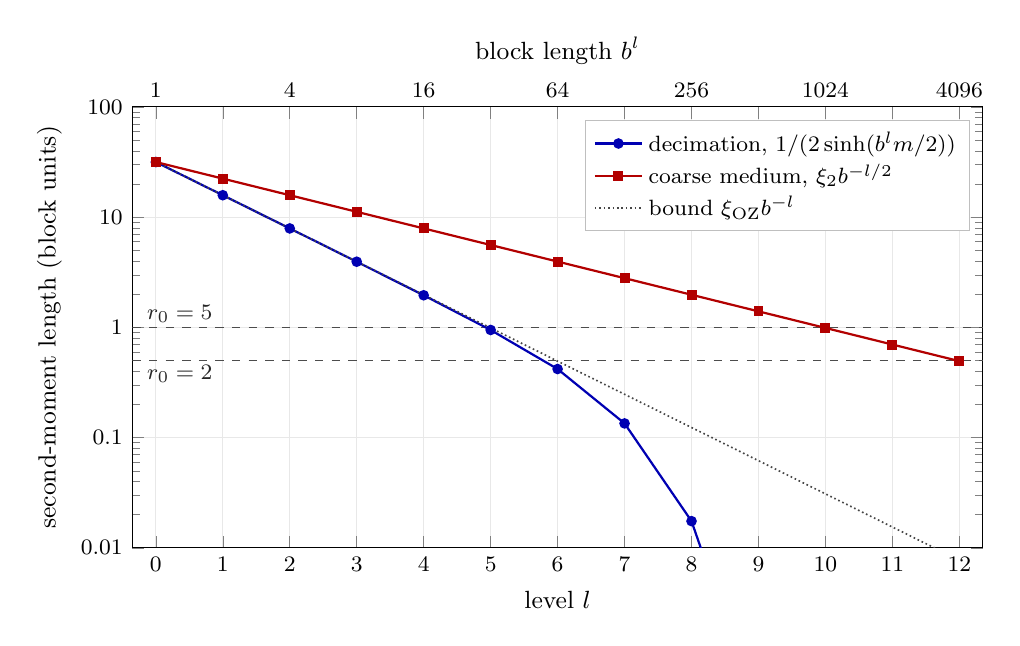
\begin{tikzpicture}
  \begin{semilogyaxis}[name=len, width=10.8cm, height=5.6cm, scale only axis,
      xmin=-0.35, xmax=12.35, ymin=0.01, ymax=100,
      xtick={0,...,12}, ytick={0.01,0.1,1,10,100}, log ticks with fixed point,
      grid=major, grid style={gray!18},
      xlabel={level $l$}, ylabel={second-moment length (block units)},
      every axis label/.style={font=\small}, tick label style={font=\footnotesize},
      legend style={font=\footnotesize, at={(0.985,0.97)}, anchor=north east, draw=gray!50, fill=white,
        cells={anchor=west}, row sep=-1pt}]
    \draw[gray!60!black, dashed] (axis cs:-0.35,1) -- (axis cs:12.35,1);
    \draw[gray!60!black, dashed] (axis cs:-0.35,0.5) -- (axis cs:12.35,0.5);
    \addplot[blue!70!black, thick, mark=*, mark size=1.5pt] coordinates {(0,31.6228) (1,15.8094) (2,7.90076)
      (3,3.94249) (4,1.95558) (5,0.947317) (6,0.418891) (7,0.134505) (8,0.0174705) (9,0.000305032)};
    \addlegendentry{decimation, $1/(2\sinh(b^lm/2))$}
    \addplot[red!70!black, thick, mark=square*, mark size=1.4pt] coordinates {(0,31.6228) (1,22.3607) (2,15.8114)
      (3,11.1803) (4,7.90569) (5,5.59017) (6,3.95285) (7,2.79508) (8,1.97642) (9,1.39754) (10,0.988212)
      (11,0.698771) (12,0.494106)};
    \addlegendentry{coarse medium, $\xi_2b^{-l/2}$}
    \addplot[gray!55!black, densely dotted, semithick] coordinates {(0,31.6241) (1,15.812) (2,7.90602) (3,3.95301)
      (4,1.97651) (5,0.988253) (6,0.494126) (7,0.247063) (8,0.123532) (9,0.0617658) (10,0.0308829)
      (11,0.0154415) (12,0.00772073)};
    \addlegendentry{bound $\xi_{\mathrm{OZ}}b^{-l}$}
    \node[font=\footnotesize, gray!30!black, anchor=south west, inner sep=1.5pt] at (axis cs:-0.2,1) {$r_0=5$};
    \node[font=\footnotesize, gray!30!black, anchor=north west, inner sep=1.5pt] at (axis cs:-0.2,0.5) {$r_0=2$};
  \end{semilogyaxis}
  \begin{axis}[at={(len.south west)}, anchor=south west, width=10.8cm, height=5.6cm, scale only axis,
      xmin=-0.35, xmax=12.35, ymin=0, ymax=1, axis x line*=top, axis y line=none,
      xtick={0,2,...,12}, xticklabels={$1$,$4$,$16$,$64$,$256$,$1024$,$4096$},
      xlabel={block length $b^l$},
      every axis label/.style={font=\small}, tick label style={font=\footnotesize}]
  \end{axis}
\end{tikzpicture}

  \caption{\textbf{Coarse second-moment lengths per level.} The nearest-neighbor precision on $\Z$ with $\varepsilon^\Pi/a^\Pi=10^{-3}$, for which $\cosh m=1+\varepsilon^\Pi/(2a^\Pi)$ gives $m=0.03162$ and $\xi_2=31.62$, is coarse-grained with block factor $b=2$; lengths are in units of the level-$l$ lattice, and the top axis gives the block length $b^l$. The exact law decimated $l$ times has the length $\xi^{(l)}_2=1/(2\sinh(b^lm/2))$ (\cref{thm:ren-decimation}), which follows the bound $\xi_{\mathrm{OZ}}b^{-l}$ of \cref{prop:ren-depth}(b) (dotted) while $b^lm\ll1$ and then falls exponentially. The coarse medium of blocks of side $b^l$ has the length $\xi_2b^{-l/2}$ (\cref{prop:ren-depth}(d)). The dashed lines are the thresholds $\frac12(r_0-1)^{1/2}$ of \cref{prop:ren-depth}(a) at $r_0=2$ and $r_0=5$: blocks of level $l+1$ reach contrast $r_0$ only while the length of level $l$ lies on or above them. The decimated length does so up to level $5$ for $r_0=2$ and up to level $4$ for $r_0=5$, block lengths $32$ and $16$ (\cref{chk:ren-depth}), within the bounds $b^l\le55.7$ and $b^l\le30.4$ of \cref{prop:ren-depth}(b); the coarse-medium length does so up to levels $11$ and $9$, block lengths $2048$ and $512$, within the bounds $b^l\le4000$ and $b^l\le1000$ of \cref{prop:ren-depth}(d).}
  \label{fig:ren-lengths}
\end{figure}

\subsection{Collectives across levels}\label{sec:ren-levels}

Which blocks of a hierarchy are collectives depends on the comparison medium of \cref{def:col-baseline}. For a population without declared geometry the comparison is exchangeable, and then only dense groups qualify.

For a finite closed population of $N$ agents with uniform leak and no declared geometry or coupling mechanism, the condition for a region of $n\ge2$ agents to be a collective at some admissible level is a pair of explicit inequalities, and each member of such a collective then has coupling to the other members above $\frac{(n-1)N}{n(N-1)}$ times the mean total coupling of an agent (Supplement, \cref{prop:ren-exchangeable}).

In a hierarchy, \cref{def:col-hierarchy} judges the blocks of level $l+1$ in the coarse medium of level $l$, against that medium's own comparison medium. For the nested medium, which declares no geometry at any level, the judgment has a closed form. Put $S_m=\sum_{j=1}^m\mathfrak q^{j-1}$, $M=b^m$ and
\[
\Delta_{\mathrm H}(b,\mathfrak q,m)=\frac b{b-1}-(S_m-1)-\frac M{M-1}S_m,\qquad T_{\mathrm H}(b,\mathfrak q,m)=\frac{MS_m(S_m-1)}{(M-1)\Delta_{\mathrm H}(b,\mathfrak q,m)}.
\]

In these terms, with the exchangeable comparison at every level, the level-$(l+1)$ blocks are collectives of the level-$l$ coarse medium, $0\le l\le n_{\mathrm H}-2$, if and only if $\Delta_{\mathrm H}(b,\mathfrak q,n_{\mathrm H}-l)>0$ and $\varepsilon^\Pi/(A_{\mathrm h}\mathfrak q^l)>T_{\mathrm H}(b,\mathfrak q,n_{\mathrm H}-l)$; nested collectives exist at every level if and only if $\mathfrak q<b/(2b^2-1)$ and the leak exceeds the largest of these thresholds, and at no level when $\mathfrak q\ge1/(2b-1)$ (Supplement, \cref{prop:ren-per-level}; \cref{fig:ren-per-level}).

\begin{figure}[!t]
  \centering
  % Figure: nested collectives judged level by level (prop:ren-per-level, thm:ren-nested), exchangeable comparison at
% every level. With S_m = sum_{j=1}^m q^{j-1}, M = b^m:
% Delta_H(b,q,m) = b/(b-1) - (S_m - 1) - M S_m/(M-1),  T_H(b,q,m) = M S_m (S_m - 1)/((M-1) Delta_H(b,q,m)).
% The level-(l+1) blocks are collectives of the level-l coarse medium iff Delta_H(b,q,n_H - l) > 0 and
% eps/(A_h q^l) > T_H(b,q,n_H - l) (prop:ren-per-level(b)).
% (a) The (b,q) plane, b in [2,5], logarithmic q axis; curves drawn through the integer values of b.
% Solid: q = b/(2b^2-1), the zero set of Delta_H at m = 2 (prop:ren-per-level(c): Delta_H > 0 for every m >= 2 iff
% q < b/(2b^2-1)). Dash-dotted: q = 1/(2b-1), the limit of the zero sets as m -> infinity, since
% Delta_H(b,q,m) = (2b-1)/(b-1) - 2/(1-q) + 2q^m/(1-q) - S_m/(b^m-1) tends to (2b-1)/(b-1) - 2/(1-q). On this curve
% Delta_H = 2q^m/(1-q) - S_m/(b^m-1) < 0 for every m >= 2: at m = 2 it equals -1/((2b-1)(b+1)); for m >= 3,
% S_m > 1 and (b-1)(2b-1)^{m-1} >= b^m. Delta_H decreases in q, so it is negative for every m above the curve and
% positive for all large m below it. Between the two curves the roots q_m(b) of Delta_H increase with m
% (q_2 = 0.2857, q_3 = 0.3062, q_8 = 0.3321, limit 1/3 for b = 2), so the levels with m = n_H - l large, the lower
% levels, qualify and the top level never does; prop:ren-per-level(f) proves that Delta_H increases strictly in
% m >= 2 for q < 1/(2b-1) and is negative for every m >= 2 for q >= 1/(2b-1). Dashed: q = 1/b (prop:ren-per-level(d): no level for q >= 1/b);
% the band 1/b < q < 1 is the power-law coherence of prop:abs-hierarchy(b). On 1789209 triples (b = 2..10,
% q = 0.001..0.999, m = 2..200) the sign pattern of Delta_H has no exception to these regions; the roots for
% m = 2..80 increase with m and stay below 1/(2b-1).
% Dot: the medium (b,q) = (2,0.2) of panel (b). Circles: the media (b,q) = (3,0.5), (2,0.7), (4,0.3) of
% chk:ren-per-level, in which no level qualified at any of 121 leaks in [1e-4,1e2].
% (b) (b,n_H,A_h,q) = (2,8,1,0.2): thresholds A_h q^l T_H(2,0.2,8-l) for l = 0..6 are 0.633645, 0.128496,
% 0.0264273, 0.00559337, 0.00125528, 3.17440e-4, 1.02400e-4 (T_H = 0.6336, 0.6425, 0.6607, 0.6992, 0.7845, 0.9920,
% 1.6000; Delta_H = 0.4951, ..., 0.2000). Bars: leaks at which the level-(l+1) blocks are collectives of the level-l
% coarse medium. Dashed: every level for eps > 0.633645, the binding level being l = 0. Recomputed from the explicit
% medium on 256 agents with coarse media Q Pi^(l) Q^T (sum convention, unit leak 2^l eps): lambda_2, cut per member
% and mean coupling equal the closed forms, the thresholds agree to 6.2e-11 relative, and on 121 leaks log-spaced in
% [1e-4,1e2] the first qualifying leak of each level is the first grid point above its threshold.
\begin{tikzpicture}
  \pgfplotsset{levelframe/.style={scale only axis, height=6.0cm,
      every axis label/.style={font=\small}, tick label style={font=\footnotesize}}}
  % panel (a): the (b, q) plane
  \begin{semilogyaxis}[levelframe, name=pa, width=6.3cm, xmin=2, xmax=5, ymin=0.08, ymax=1,
      xtick={2,...,5}, ytick={0.1,0.2,0.5,1}, log ticks with fixed point, axis on top, clip=false,
      xlabel={branching $b$}, ylabel={allocation $\mathfrak q$}]
    \addplot[draw=none, fill=green!20, forget plot] coordinates {(2,0.08) (2,0.285714) (2.125,0.264591) (2.25,0.246575) (2.375,0.231003) (2.5,0.217391) (2.625,0.205379)
      (2.75,0.19469) (2.875,0.185111) (3,0.176471) (3.125,0.168634) (3.25,0.161491) (3.375,0.15495) (3.5,0.148936)
      (3.625,0.143387) (3.75,0.138249) (3.875,0.133477) (4,0.129032) (4.125,0.124882) (4.25,0.120996) (4.375,0.117351)
      (4.5,0.113924) (4.625,0.110696) (4.75,0.107649) (4.875,0.104768) (5,0.102041) (5,0.08)} -- cycle;
    \addplot[draw=none, fill=yellow!50, forget plot] coordinates {(2,0.285714) (2.125,0.264591) (2.25,0.246575) (2.375,0.231003) (2.5,0.217391) (2.625,0.205379) (2.75,0.19469)
      (2.875,0.185111) (3,0.176471) (3.125,0.168634) (3.25,0.161491) (3.375,0.15495) (3.5,0.148936) (3.625,0.143387)
      (3.75,0.138249) (3.875,0.133477) (4,0.129032) (4.125,0.124882) (4.25,0.120996) (4.375,0.117351) (4.5,0.113924)
      (4.625,0.110696) (4.75,0.107649) (4.875,0.104768) (5,0.102041) (5,0.111111) (4.875,0.114286) (4.75,0.117647)
      (4.625,0.121212) (4.5,0.125) (4.375,0.129032) (4.25,0.133333) (4.125,0.137931) (4,0.142857) (3.875,0.148148)
      (3.75,0.153846) (3.625,0.16) (3.5,0.166667) (3.375,0.173913) (3.25,0.181818) (3.125,0.190476) (3,0.2)
      (2.875,0.210526) (2.75,0.222222) (2.625,0.235294) (2.5,0.25) (2.375,0.266667) (2.25,0.285714) (2.125,0.307692)
      (2,0.333333)} -- cycle;
    \addplot[draw=none, fill=orange!15, forget plot] coordinates {(2,0.5) (2.125,0.470588) (2.25,0.444444) (2.375,0.421053) (2.5,0.4) (2.625,0.380952) (2.75,0.363636)
      (2.875,0.347826) (3,0.333333) (3.125,0.32) (3.25,0.307692) (3.375,0.296296) (3.5,0.285714) (3.625,0.275862)
      (3.75,0.266667) (3.875,0.258065) (4,0.25) (4.125,0.242424) (4.25,0.235294) (4.375,0.228571) (4.5,0.222222)
      (4.625,0.216216) (4.75,0.210526) (4.875,0.205128) (5,0.2) (5,1) (2,1)} -- cycle;
    \addplot[black, thick] coordinates {(2,0.285714) (2.125,0.264591) (2.25,0.246575) (2.375,0.231003) (2.5,0.217391) (2.625,0.205379) (2.75,0.19469)
      (2.875,0.185111) (3,0.176471) (3.125,0.168634) (3.25,0.161491) (3.375,0.15495) (3.5,0.148936) (3.625,0.143387)
      (3.75,0.138249) (3.875,0.133477) (4,0.129032) (4.125,0.124882) (4.25,0.120996) (4.375,0.117351) (4.5,0.113924)
      (4.625,0.110696) (4.75,0.107649) (4.875,0.104768) (5,0.102041)};
    \addplot[black, thick, dashdotted] coordinates {(2,0.333333) (2.125,0.307692) (2.25,0.285714) (2.375,0.266667) (2.5,0.25) (2.625,0.235294) (2.75,0.222222)
      (2.875,0.210526) (3,0.2) (3.125,0.190476) (3.25,0.181818) (3.375,0.173913) (3.5,0.166667) (3.625,0.16)
      (3.75,0.153846) (3.875,0.148148) (4,0.142857) (4.125,0.137931) (4.25,0.133333) (4.375,0.129032) (4.5,0.125)
      (4.625,0.121212) (4.75,0.117647) (4.875,0.114286) (5,0.111111)};
    \addplot[black, thick, dashed] coordinates {(2,0.5) (2.125,0.470588) (2.25,0.444444) (2.375,0.421053) (2.5,0.4) (2.625,0.380952) (2.75,0.363636)
      (2.875,0.347826) (3,0.333333) (3.125,0.32) (3.25,0.307692) (3.375,0.296296) (3.5,0.285714) (3.625,0.275862)
      (3.75,0.266667) (3.875,0.258065) (4,0.25) (4.125,0.242424) (4.25,0.235294) (4.375,0.228571) (4.5,0.222222)
      (4.625,0.216216) (4.75,0.210526) (4.875,0.205128) (5,0.2)};
    % region labels
    \node[font=\footnotesize] at (axis cs:3.0,0.11) {every level};
    \path (axis cs:2.115,0.28491) -- node[sloped, font=\footnotesize, inner sep=0pt]
      {lower levels} (axis cs:2.785,0.203387);
    \node[font=\footnotesize] at (axis cs:4.45,0.175) {no level};
    \node[font=\footnotesize, align=center] at (axis cs:3.95,0.55) {power-law coherence,\\no level};
    % curve labels, along the curves
    \path (axis cs:3.95,0.130773) -- node[sloped, below, font=\footnotesize, inner sep=2pt]
      {$\mathfrak q=b/(2b^2-1)$} (axis cs:4.75,0.107649);
    \path (axis cs:3.3,0.178571) -- node[sloped, above, font=\footnotesize, inner sep=2pt]
      {$\mathfrak q=1/(2b-1)$} (axis cs:4.0,0.142857);
    \path (axis cs:4.1,0.243902) -- node[sloped, above, font=\footnotesize, inner sep=2pt]
      {$\mathfrak q=1/b$} (axis cs:4.7,0.212766);
    % media
    \addplot[only marks, mark=*, mark size=1.7pt, black] coordinates {(2,0.2)};
    \node[font=\footnotesize, anchor=north west, inner sep=1pt] at (axis cs:2.04,0.19) {(b)};
    \addplot[only marks, mark=*, mark size=1.7pt, black, mark options={fill=white}] coordinates {(3,0.5) (2,0.7)
      (4,0.3)};
  \end{semilogyaxis}
  \node[font=\small\bfseries, anchor=south east] at ($(pa.north west)+(-0.25cm,0.05cm)$) {(a)};
  % panel (b): leak thresholds per level
  \begin{semilogyaxis}[levelframe, name=pb, at={($(pa.south east)+(2.0cm,0)$)}, anchor=south west,
      width=5.4cm, xmin=-0.8, xmax=6.6, ymin=5e-5, ymax=3, xtick={0,...,6},
      ytick={1e-4,1e-3,1e-2,1e-1,1}, grid=major, grid style={gray!18},
      xlabel={coarse level $l$}, ylabel={leak $\varepsilon^\Pi$}]
    \fill[green!20] (axis cs:-0.2,0.633645) rectangle (axis cs:0.2,3);
    \fill[green!20] (axis cs:0.8,0.128496) rectangle (axis cs:1.2,3);
    \fill[green!20] (axis cs:1.8,0.0264273) rectangle (axis cs:2.2,3);
    \fill[green!20] (axis cs:2.8,0.00559337) rectangle (axis cs:3.2,3);
    \fill[green!20] (axis cs:3.8,0.00125528) rectangle (axis cs:4.2,3);
    \fill[green!20] (axis cs:4.8,0.00031744) rectangle (axis cs:5.2,3);
    \fill[green!20] (axis cs:5.8,0.0001024) rectangle (axis cs:6.2,3);
    \draw[gray!60!black, dashed] (axis cs:-0.8,0.633645) -- (axis cs:6.6,0.633645);
    \addplot[only marks, mark=*, mark size=1.6pt, black] coordinates {(0,0.633645) (1,0.128496)
      (2,0.0264273) (3,0.00559337) (4,0.00125528) (5,0.00031744) (6,0.0001024)};
    \node[font=\footnotesize, anchor=north, inner sep=3pt] at (axis cs:0,0.633645) {$0.6336$};
    \node[font=\footnotesize, anchor=east, inner sep=3.5pt] at (axis cs:1,0.128496) {$0.1285$};
    \node[font=\footnotesize, anchor=east, inner sep=3.5pt] at (axis cs:2,0.0264273) {$0.02643$};
    \node[font=\footnotesize, anchor=east, inner sep=3.5pt] at (axis cs:3,0.00559337) {$0.005593$};
    \node[font=\footnotesize, anchor=east, inner sep=3.5pt] at (axis cs:4,0.00125528) {$0.001255$};
    \node[font=\footnotesize, anchor=east, inner sep=3.5pt] at (axis cs:5,0.00031744) {$3.174\times10^{-4}$};
    \node[font=\footnotesize, anchor=east, inner sep=3.5pt] at (axis cs:6,0.0001024) {$1.024\times10^{-4}$};
    \node[font=\footnotesize, anchor=south east, inner sep=1.5pt] at (axis cs:6.35,0.68) {every level};
  \end{semilogyaxis}
  \node[font=\small\bfseries, anchor=south east] at ($(pb.north west)+(-0.25cm,0.05cm)$) {(b)};
\end{tikzpicture}

  \caption{\textbf{Nested collectives judged level by level.} The nested medium of \cref{thm:ren-nested} with the exchangeable comparison at every level (Supplement, \cref{prop:ren-per-level}). (a) The plane of the branching $b$ and the allocation $\mathfrak q$, with the curves drawn through the integer values of $b$. Below the solid curve $\mathfrak q=b/(2b^2-1)$, $\Delta_{\mathrm H}(b,\mathfrak q,m)>0$ for every $m\ge2$, and the blocks of every level are collectives above a leak threshold (\cref{prop:ren-per-level}(c)). The dash-dotted curve $\mathfrak q=1/(2b-1)$ is the limit of the zero sets of $\Delta_{\mathrm H}(b,\mathfrak q,m)$ as $m\to\infty$. Between the two curves $\Delta_{\mathrm H}(b,\mathfrak q,2)\le0$ while $\Delta_{\mathrm H}(b,\mathfrak q,m)$ increases with $m$ and is positive for all large $m$, so the top level is never a collective and the lower levels of a deep enough hierarchy are, above a leak threshold; above the dash-dotted curve $\Delta_{\mathrm H}<0$ for every $m$, and no level is (\cref{prop:ren-per-level}(f)). This includes the range $\mathfrak q\ge1/b$ of \cref{prop:ren-per-level}(d) (dashed curve), where \cref{prop:abs-hierarchy}(b) gives power-law coherence for $\mathfrak q<1$. The dot marks the medium of panel (b), and the circles the media $(b,\mathfrak q)=(3,0.5)$, $(2,0.7)$ and $(4,0.3)$ of \cref{chk:ren-per-level}, in which no level qualified at any of $121$ leaks in $[10^{-4},10^2]$. (b) For $(b,n_{\mathrm H},A_{\mathrm h},\mathfrak q)=(2,8,1,0.2)$ the level-$(l+1)$ blocks are collectives of the level-$l$ coarse medium at the leaks above $A_{\mathrm h}\mathfrak q^lT_{\mathrm H}(b,\mathfrak q,n_{\mathrm H}-l)$ (bars), whose values for $l=0,\dots,6$ are $0.6336$, $0.1285$, $0.02643$, $0.005593$, $0.001255$, $3.174\times10^{-4}$ and $1.024\times10^{-4}$; they fall like $\mathfrak q^l$, while $T_{\mathrm H}$ rises from $0.634$ at $l=0$ to $1.6$ at $l=6$. The largest, at $l=0$, is the leak $0.6336$ above which collectives exist at every level (dashed line).}
  \label{fig:ren-per-level}
\end{figure}

\subsection{Memory and the adiabatic reduction}\label{sec:ren-memory}

\Cref{thm:agy-closure-average} treats one collective with its exterior held fixed. A coarse-grained population is a set of blocks whose exteriors are the other blocks, so we need the joint version. Let $\varpi_1\le\varpi_2\le\cdots$ be the eigenvalues of $\Pi$, let $\mathsf V_{\mathrm s}$ and $\mathsf V_{\mathrm f}$ hold orthonormal eigenvectors of the $M$ smallest and of the others, let $\varkappa_\Phi=\lambda_{\max}(\Pi_\Phi)$, and put $\mathsf t_\Theta=\Vert\Pi_{\perp\Phi}\Vert/(\varkappa_\perp-\varkappa_\Phi)$.

\begin{theorem}[Exact reduction of a partitioned reversible population]\label{thm:ren-memory}
Let $\Pi\succ0$ be symmetric, let $x$ follow $\mathrm dx=-\Pi x\mathrm dt+\sqrt2\mathrm d\mathsf B_t$ in its stationary law, let $\Phi\in\R^{N\times M}$ have orthonormal columns, and let $y=\Phi^\top x$.
\begin{enumerate}
\item[(a)] (Static law.) $\Cov(y)^{-1}=\Pi_\Phi-\mathcal D$, with $\mathcal D$ as in \cref{lem:ren-galerkin}.
\item[(b)] (Memory.) $\dot y(t)=-\Pi_\Phi y(t)+\int_0^t\Gamma(t-t')y(t')\mathrm dt'+\mathfrak f(t)$, with kernel $\Gamma(u)=\Pi_{\perp\Phi}^\top e^{-\Pi_{\perp\perp}u}\Pi_{\perp\Phi}\succeq0$, $\Vert\Gamma(u)\Vert\le\Vert\Pi_{\perp\Phi}\Vert^2e^{-\varkappa_\perp u}$ and $\int_0^\infty\Gamma(u)\mathrm du=\mathcal D$: the static correction of the bridge theorem is the integrated memory kernel.
\item[(c)] (Slow and fast parts.) If $\varkappa_\perp>\varkappa_\Phi$, then $\varpi_M\le\varkappa_\Phi<\varkappa_\perp\le\varpi_{M+1}$, and the largest principal angle $\Theta$ between $\operatorname{range}\Phi$ and $\operatorname{range}\mathsf V_{\mathrm s}$ satisfies $\sin\Theta\le\mathsf t_\Theta$. If $\mathsf t_\Theta<1$, then exactly $y=\mathsf Tz_{\mathrm s}+y_{\mathrm f}$, where $z_{\mathrm s}=\mathsf V_{\mathrm s}^\top x$ is an Ornstein--Uhlenbeck process with drift $\diag(\varpi_1,\dots,\varpi_M)$, $\mathsf T=\Phi^\top\mathsf V_{\mathrm s}$ is invertible, and $y_{\mathrm f}$ is independent of $z_{\mathrm s}$, has an autocovariance that decays at rates at least $\varkappa_\perp$, and has relative weight $\Vert\Cov(y)^{-1/2}\Cov(y_{\mathrm f})\Cov(y)^{-1/2}\Vert\le\mathsf t_\Theta^2\varkappa_\Phi/\varkappa_\perp$. The slow part is exactly Markov, with drift $\mathsf T\diag(\varpi_1,\dots,\varpi_M)\mathsf T^{-1}$, which differs from $\Pi_\Phi$ by at most $\Vert\Pi_{\perp\Phi}\Vert\mathsf t_\Theta/(1-\mathsf t_\Theta^2)^{1/2}$ in norm.
\item[(d)] (Contrast.) For the block indicators of a partition into regions $C_1,\dots,C_M$ of a diffusive $\Pi$, whose leaks need not be uniform, $\varkappa_\perp\ge\xin^{\min}$, the minimum of $\xin(C_j)$ over the regions with at least two members (the bounds are vacuous if every region is a singleton), $\varkappa_\Phi\le\max_j(2\xout(C_j)-\bar\varepsilon_{C_j})$, which for uniform leak $\varepsilon^\Pi$ is $2\xout^{\max}-\varepsilon^\Pi$ with $\xout^{\max}=\max_j\xout(C_j)$, and $\Vert\Pi_{\perp\Phi}\Vert\le\sigma_{\mathrm{cut}}$. If $\xin^{\min}>\max_j(2\xout(C_j)-\bar\varepsilon_{C_j})$, every bound of (a) to (c) holds with $\varkappa_\perp-\varkappa_\Phi\ge\xin^{\min}-\max_j(2\xout(C_j)-\bar\varepsilon_{C_j})$, which for uniform leak is $\xin^{\min}-2\xout^{\max}+\varepsilon^\Pi$. If all blocks have the same rates $\xin$ and $\xout$, with contrast $r>2$, the relative fast weight is at most $2(\Vert\Pi_{\perp\Phi}\Vert/(\xout(r-2)))^2/r$.
\end{enumerate}
\end{theorem}
% src: H4-T8 (CHECKED); C3_05 recomputation (200 populations)
Proof in \cref{app:ren}; checked on $200$ random partitioned populations and on block media of square blocks (\cref{chk:ren-memory}). Part (d) is the multi-block form of the closure bound of \cref{thm:agy-h1}. Coarse-graining along collectives with $\Vert\Pi_{\perp\Phi}\Vert^2\ll\xin^{\min}\xout$ makes memory a correction of that relative order; coarse-graining across them does not. The spectral norm is the intensive measure: for $M$ identical blocks $\sigma^2_{\mathrm{cut}}$ grows in proportion to $M$, while $\Vert\Pi_{\perp\Phi}\Vert$ and $\Vert\mathcal D\Vert$ do not (\cref{chk:ren-memory}).

The adiabatic reduction of \citet{friston2019free}, read in its primary text, builds scales with two operators. A grouping operator $G$ forms a particular partition into particles from the coupling structure of the Jacobian and eliminates internal states by conditioning on blankets, absorbing their fluctuations into those of the next level; a reduction operator $R$ keeps the slow eigenmodes of each particle's own blanket Jacobian as the states of the next level and absorbs the fast ones into fluctuations. An ensemble assumption takes the slow and fast modes of different particles to be uncoupled, correlations among the induced fluctuations are set aside, and $R\circ G$ is read as a renormalization that preserves the functional form of the dynamics, with slower modes and smaller fluctuations at each level. The linear reversible analogue of $R$ is a frame of per-particle slowest modes.

\begin{proposition}[Per-particle slow modes]\label{prop:ren-perron}
In the setting of \cref{thm:ren-memory}, let a partition into particles $C_1,\dots,C_M$ be given, let $\mathsf u_j$ be a unit eigenvector of the smallest eigenvalue of $\Pi_{C_jC_j}$, the slowest mode of particle $j$'s own drift, which is positive by the Perron--Frobenius theorem when $\Pi$ is diffusive and $C_j$ is connected, and let $\Phi^{\mathsf P}=\diag(\mathsf u_1,\dots,\mathsf u_M)$. The reduction AR0, $\mathrm dy=-\Pi_{\Phi^{\mathsf P}}y\mathrm dt+\sqrt2\mathrm d\mathsf W_t$ with $\mathsf W$ a standard Brownian motion, discards the fast modes.
\begin{enumerate}
\item[(a)] AR0 is exact, in law and in dynamics, if and only if $\Pi_{C_kC_j}\mathsf u_j\in\operatorname{span}\mathsf u_k$ for all $j\neq k$: the slow mode of each particle drives the other particles only along their slow modes. This is the ensemble assumption in linear form; within a particle it holds automatically.
\item[(b)] Otherwise the stationary precision of AR0 errs by exactly $\mathcal D^{\mathsf P}$, the matrix $\mathcal D$ of the frame $\Phi^{\mathsf P}$, and \cref{thm:ren-memory} applies with $\Vert\Pi_{\perp\Phi^{\mathsf P}}\Vert$, which collects only couplings from the slow mode of one particle to fast modes of others. The Markov reduction that matches the stationary law and the short-time derivative of the autocovariance of $y$ has drift $\Pi_{\Phi^{\mathsf P}}-\mathcal D^{\mathsf P}$ and unit noise; its only error is the memory of \cref{thm:ren-memory}(b).
\item[(c)] Per-particle modes miss the global slow mode: with uniform leak the slowest mode $\one/N^{1/2}$, of rate $\varepsilon^\Pi$, lies in the span of the block indicators but not in $\operatorname{range}\Phi^{\mathsf P}$ unless every $\mathsf u_j$ is constant. If $\varkappa_\perp$, computed in the frame $\Phi^{\mathsf P}$, exceeds $\lambda_{\min}(\Pi_{\Phi^{\mathsf P}})$, then $0\le\lambda_{\min}(\Pi_{\Phi^{\mathsf P}})-\varepsilon^\Pi\le\Vert\Pi_{\perp\Phi^{\mathsf P}}\Vert^2/(\varkappa_\perp-\lambda_{\min}(\Pi_{\Phi^{\mathsf P}}))$, while $\lambda_{\min}(\Pi_\Phi)=\varepsilon^\Pi$ exactly for block averages.
\item[(d)] For equal blocks, $M^{-1}\tr\Pi_\Phi=N^{-1}\sum_i(\varepsilon^\Pi_i+a^\partial_i)\le N^{-1}\tr\Pi$, with $a^\partial_i$ the coupling of agent $i$ to other blocks, and $\tr(\Pi_\Phi-\mathcal D)\le\tr\Pi_\Phi$: block averages are slower on average. Whether fluctuations become smaller depends on the normalization: block averages have variance at most $\lambda_{\max}(\Sigma)/\lvert X\rvert$, while the normalization that keeps the coarse coupling fixed leaves the noise intensity unchanged.
\end{enumerate}
\end{proposition}
% src: H4-P9 (CHECKED); C3_05 recomputation; H4-R2 and H1-R1 merged on the operators per HC_critic Section 4 (G eliminates, R keeps slow eigenmodes)
Proof in \cref{app:ren}; checked on block media in \cref{chk:ren-perron}, where at contrast $35.1$ the Perron frame couples the particles more weakly than the frame of block averages, but its slowest retained rate is $1.0368\times10^{-3}$ against the exact $10^{-3}$. Without contrast the Galerkin description fails at leading order.

For the nearest-neighbor precision on $\Z$ and blocks of $b$ sites the coarse medium overstates the squared second-moment length of the block averages, in block units, by a factor that tends to $b$ as the leak vanishes, and averaged update weights overstate the coarse message weight by the same factor up to corrections of order the leak (Supplement, \cref{ex:ren-no-contrast}).

The grouping step $G$, the elimination of internal states, drops a memory kernel, an initial-state term and the color of the force from an exact equation for the retained states, those that are not internal, which are Markov with a transition law independent of the initial law if and only if no retained state is driven by an internal one (Supplement, \cref{prop:ren-adiabatic}, for stable linear dynamics on a particular partition, under the hypotheses stated there). The size of what is dropped is a numerical observation without a proved rate (\cref{obs:ren-adiabatic-rate}), and \cref{rem:ren-rgm} compares renormalizing generative models.

\subsection{The framework under coarse-graining}\label{sec:ren-closure}

Codes, relay ranks, decision dimensions and interpretation levels under aggregation are treated in the Supplement (\cref{sec:ren-codes}). A meta-agent $J$ that aggregates the public messages of its members with weights $\mathsf w_j\ge0$ that sum to one has the aggregate code $T_c\bar U_J$, with $\bar U_J=\sum_{j\in J}\mathsf w_jU_j$. Aggregation in public coordinates never raises the rank of a code, and aggregation after true translation loses nothing (\cref{prop:ren-codes,prop:ren-code-levels}); under the hypotheses stated there, the effective rank of stationary averaged relays is nonincreasing along the relay and the Hayek dimension is nonincreasing up the hierarchy (\cref{prop:ren-relay-rank,prop:ren-hayek}); and literal reading in a regular hierarchy counts the common prior once per agent in the limit of many rounds, while consensus on information contributions that passes exact sums upward and adds the common prior once at the top returns the union posterior (\cref{prop:ren-literal-levels}).

For networks without coordinates the Supplement (\cref{sec:ren-network}) compares contrast with the Laplacian renormalization group of \citet{villegas2023laplacian}. With uniform leak that procedure does not depend on the leak, whereas contrast does (\cref{prop:ren-lrg}); the two agree on an interval of leaks for a population formed by two blocks of equal size with an equitable cut and equal internal gaps, under the gap condition stated there (\cref{prop:ren-lrg-agreement}); in an example with interleaved scales no single diffusion time returns every set that contrast selects (\cref{ex:ren-interleaved}); and which regions of high ratio the procedure returns is an open problem (\cref{conj:ren-lrg}).

\begin{theorem}[What coarse-graining preserves]\label{thm:ren-closure}
Let a population satisfy \cref{asm:ren-standing}, and let a partition $\mathcal X$ into blocks, the candidate meta-agents, be coarse-grained by block averaging.
\begin{enumerate}
\item[(a)] (Static law.) The block coordinates have the Gaussian precision $\Pi_\Phi-\mathcal D$ (\cref{lem:ren-galerkin}); whether or not the leak is uniform, $\Vert\mathcal D\Vert\le\Vert\Pi_{\perp\Phi}\Vert^2/\xin^{\min}\le\sigma^2_{\mathrm{cut}}/\xin^{\min}$ and $\lvert\mathcal D_{XY}\rvert\le\sigma_X\sigma_Y/\xin^{\min}$, with $\xin^{\min}$ the minimum of $\xin(X)$ over the blocks with at least two members (the bounds are vacuous if every block is a singleton), and these bound the departure from $\Pi_\Phi$ of the exact law, which is in general not diffusive (\cref{ex:ren-block-average}). For uniform leak $\mathcal D$ also leaves the leak unchanged (\cref{lem:ren-galerkin}(c)).
\item[(b)] (Coarse level-0 network.) Under $e(t+1)=We(t)+\zeta(t)$ the block averages obey $\bar e(t+1)=W^{(1)}\bar e(t)+\diag(\lvert X\rvert)^{-1}\mathsf PWe_\perp(t)+\bar\zeta(t)$, with $e_\perp=e-\mathsf P^\top\bar e$ and $W^{(1)}=\diag(\lvert X\rvert)^{-1}\mathsf PW\mathsf P^\top$, whose entry $W^{(1)}_{XY}$ is the mean total weight that a member of $X$ places on $Y$. The matrix $W^{(1)}$ is nonnegative if $W$ is, and its row sums are block means of row sums, so the coarse leak is the mean leak and \textup{(C$_r$)} and \textup{(M)} are inherited; if the local noises satisfy \textup{(B)} of \cref{asm:sca-standing}, the $\bar\zeta_X$ are independent, with variance at most $q/\lvert X\rvert$, and equal to $q/\lvert X\rvert$ when every local noise has variance $q$. The memory term vanishes for every $e_\perp$ if and only if the partition is lumpable for $W$ (\cref{def:met-lumpable}), and then the coarse population is exactly a level-0 network; otherwise the exact reduction is \cref{thm:agy-mori-zwanzig}, with the bounds of \cref{thm:ren-memory} in continuous time and, for one coordinate of a reversible recursion, of \cref{lem:met-discrete-closure}.
\item[(c)] (Contrast between meta-agents.) For blocks of equal size and uniform leak, every set $S$ of at least two blocks has coarse contrast $r^{(1)}(S)\ge r(\bigcup S)$, with equality if and only if a slowest internal mode of $\bigcup S$ is constant on blocks, as at every level of the nested medium (\cref{thm:ren-nested}(c)). Hence if $\bigcup S$ is a collective of the fine medium at level $r_0$, then $S$ is a collective of the coarse medium at the same level whenever $r_0$ exceeds the coarse baseline $\bar r^{(1)}_{\mathrm{hom}}$ (\cref{def:col-hierarchy}). Under the exchangeable clause at both levels, with $N$ agents in blocks of $s$, $\bar r^{(1)}_{\mathrm{hom}}-1=\frac{N-1}{N-s}\cdot\frac{\bar c}{\bar d}(\bar r_{\mathrm{hom}}-1)$, with $\bar d$ the mean total coupling of an agent and $\bar c$ its mean coupling to other blocks, so the coarse baseline is the lower one exactly when $\bar c/\bar d\le(N-s)/(N-1)$.
\item[(d)] (Codes and interpretation.) Codes and interpretation levels transform as in \cref{prop:ren-codes,prop:ren-code-levels,prop:ren-literal-levels}: aggregation after true translation preserves codes, and the information form is closed while literal reading compounds.
\item[(e)] (Records.) In the record model of \cref{def:fw-record-model} the record equation closes exactly for block averages, $\bar z_{k,X}(t+1)=\omega_k\bar e_X(t)+(1-\omega_k-\delta_k)\bar z_{k,X}(t)+\bar\zeta^z_{k,X}(t)$, so $\beta_k$, $\omega_k$, $\delta_k$ and $\upsilon_k$ do not renormalize and record noise becomes $q_z/\lvert X\rvert$; the read term closes exactly for local records ($\ell_{r,k}=0$) and, at range, on record fields constant on blocks, with the kernel $\mathsf K^{(1)}_k(X,Y)=\lvert X\rvert^{-1}\sum_{x\in X,y\in Y}\mathsf K_k(x-y)$, a Galerkin projection otherwise; the message term keeps the memory of (b). On $\Z^D$ with cubic blocks the reduced model of the mean mode (\cref{prop:sca-records}), hence $\varepsilon_{\mathrm{rec}}$ and the correlation time of the collective mean, is the same at every level.
\item[(f)] (What fails.) Without contrast the Markov coarse coupling and squared length are wrong by the block factor $b$, up to corrections that vanish with the leak (\cref{ex:ren-no-contrast}); contrast is computed in the coarse medium, with the error of (a), because the exact law leaves the diffusive class (\cref{ex:ren-block-average}); for directed attention, discrete-time closure beyond \cref{lem:met-discrete-closure} is open, and contrast is undefined where the precision is not diffusive (\cref{open:col-non-diffusive}); without declared geometry collectives must be denser than average, and nested collectives at every level need $\mathfrak q<b/(2b^2-1)$, a leak above an explicit threshold and a declared level for each level (\cref{prop:ren-exchangeable,prop:ren-per-level}).
\end{enumerate}
\end{theorem}
% src: H4-T18 (DERIVED; parts CHECKED as cited), with (3) restated per H6-P12 and generalized here to equal blocks without equitability (checked by ren_checks.py part D), (6)(iv) replaced per H6-T2, the closure condition of (2) unified with def:met-lumpable per HC_critic V6
Proof in \cref{app:ren}; part (c) is checked on random populations with blocks that are not equitable (\cref{chk:ren-closure}), and \cref{tab:ren-parameters} lists how each parameter transforms. The framework is closed under coarse-graining exactly for partitions whose span of block indicators the precision leaves invariant, as in the nested medium; approximately, with the averaged-weight coarse parameters in error by relative order $\Vert\Pi_{\perp\Phi}\Vert^2/(\xin^{\min}\xout)$, when that ratio is small; and not even approximately for blocks without contrast. High contrast alone does not make the ratio small: for uniform leak $\sigma_X^2\le2d_{\max}(X)(\xout(X)-\varepsilon^\Pi)$ (\cref{lem:ren-galerkin}(b)), so that $\sigma_X^2/(\xin^{\min}\xout(X))\le2d_{\max}(X)/\xin^{\min}$, and this per-block ratio is small when every agent's coupling across the boundary is small against $\xin^{\min}$, as at high contrast when the cut is spread over the members; the bound gives a sufficient condition for that ratio, not a necessary one. Two cliques joined by a single strong edge have contrast that grows without bound with their size while the exact coarse coupling stays near half the averaged one (\cref{chk:ren-memory}); what survives there is the Markov property of the slow part, by \cref{thm:ren-memory}(c), with a drift that differs from $\Pi_\Phi$ at order one.

\begin{table}[t]
\centering
\caption{Parameters of the framework under block averaging (\cref{thm:ren-closure}). Lengths are in block units.}
\label{tab:ren-parameters}
\begin{tabular}{@{}p{0.25\textwidth}p{0.43\textwidth}p{0.24\textwidth}@{}}
\toprule
Parameter & Coarse value & Status\\
\midrule
uniform leak $\varepsilon$ & unchanged per base round; $b^2\varepsilon$ per coarse round of $b^2$ base rounds & exact; rescaling (\cref{prop:ren-exponents})\\
precision couplings & $\cut(X,Y)$ in the coarse medium, corrected by $\mathcal D$ & exact; $\Vert\mathcal D\Vert\le\Vert\Pi_{\perp\Phi}\Vert^2/\xin^{\min}$\\
message weights $W_{ij}$ & $W^{(1)}_{XY}$, mean total weight of a member of $X$ on $Y$ & exact if lumpable; memory otherwise\\
axis rate, $a/\varepsilon$ & rate times $b$; $a/\varepsilon$ divided by about $b^2$ & exact flow (\cref{thm:ren-flows})\\
second-moment length & divided by $b$, up to a constant & exact formula (\cref{thm:ren-flows})\\
local noise $q$ & $q/\lvert X\rvert$ & equality for equal variances; an upper bound under \textup{(B)}\\
codes $H_j$ & $T_c\bar U_X$ (public); unchanged (translated) & exact\\
record parameters & $\beta_k,\omega_k,\delta_k,\upsilon_k$ unchanged; noise $q_z/\lvert X\rvert$; kernel averaged & exact; Galerkin at range\\
interpretation level & literal: overcounting multiplies; information form: closed & exact (regular hierarchies)\\
contrast & $r^{(1)}(S)\ge r(\bigcup S)$ for equal blocks & exact inequality\\
memory & kernel at most $\Vert\Pi_{\perp\Phi}\Vert^2e^{-\xin^{\min}u}$, integral $\mathcal D$ & exact bounds\\
\bottomrule
\end{tabular}
\end{table}

Open problems beyond the exact cases, among them contrast for the non-diffusive laws of block averages and discrete-time closure for non-reversible updates, are listed in the Supplement (\cref{open:ren-beyond}).
